\section{Gestion de projet}
    L'outil de contrôle de versions retenu pour le projet est un Git hébergé par Microsoft (\url{https://github.com/mamaheux/CuriousNetwork}). Les tableaux de type Trello de GitHub ont également été utilisés pour gérer l'assignation et le suivi des tâches de développement. Un tableau a été créé pour chaque volet majeur du projet. Une vue d'ensemble des tableaux est présenté à la figure \ref{fig:trello_boards}.

    \begin{figure}[H]
        \centering
        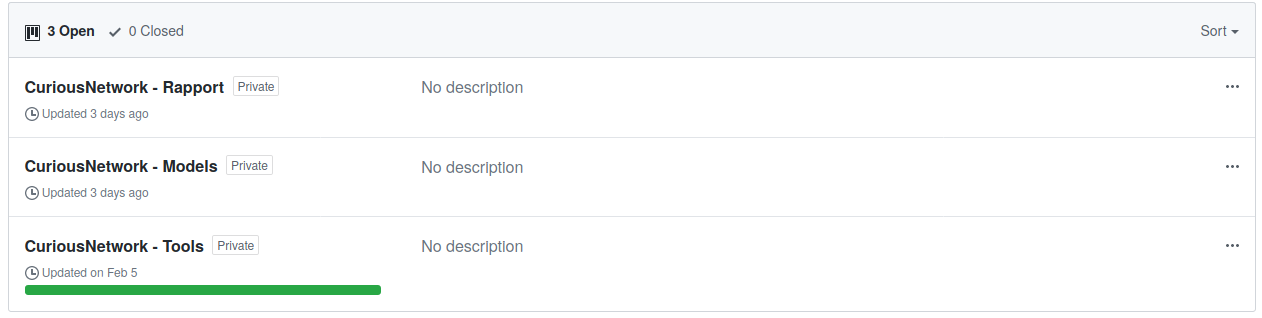
\includegraphics[width=15cm]{images/3_sub_projects.png}
        \caption{Tableaux de suivi des tâches de chaque volet du projet}
        \label{fig:trello_boards}
    \end{figure}

    La figure \ref{fig:trello_board_models} présente un aperçu du tableau de suivi pour le volet des modèles de réseaux de neurones.
    \begin{figure}[H]
        \centering
        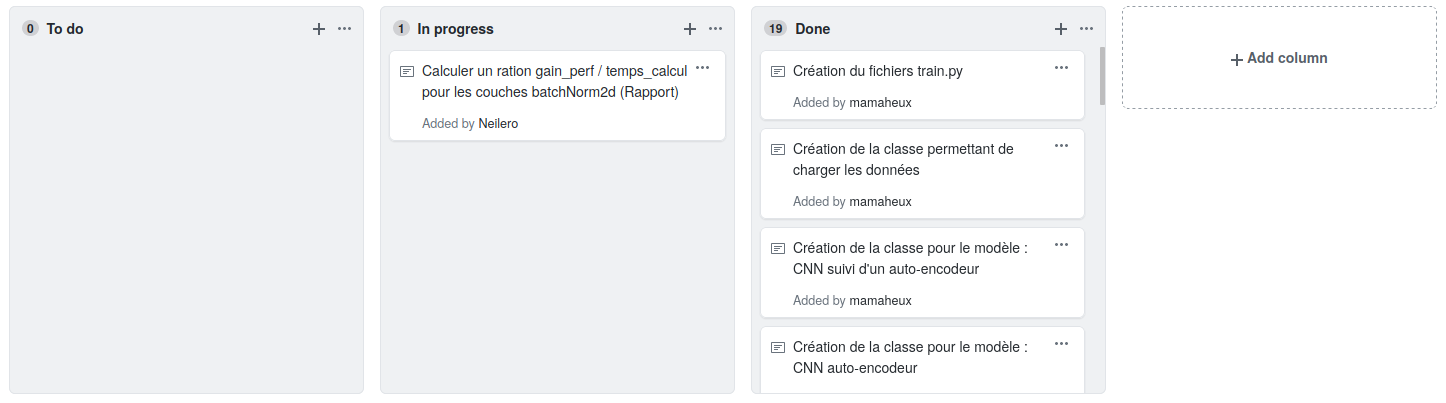
\includegraphics[width=15cm]{images/trello_board.png}
        \caption{Tableau Trello du volet \textbf{modèles}}
        \label{fig:trello_board_models}
    \end{figure}

    Pour suivre les bonnes pratiques, chaque tâche de développement a été effectuée sur sa propre branche. Une fois la tâche complétée, la branche faisait l'objet d'une demande \textit{pull request} et devait être révisée par un autre membre de l'équipe avant de pouvoir être fusionnée (\textit{merge}) à la branche principale \textit{master}. Une fois les branches fusionnées, elles étaient supprimées.\\
    
    Les \textit{commits} ont été effectués de manière à avoir la plus grande granularité possible de manière à simplifier les révisions de codes ainsi que la traçabilité. Il a été décidé de ne pas utiliser de \textit{squash and merge} afin de conserver l'historique de l'évolution du code pour chaque fusion. La figure \ref{fig:git_graph} présente un aperçu de l'arborescence Git du projet.
    \begin{figure}[H]
        \centering
        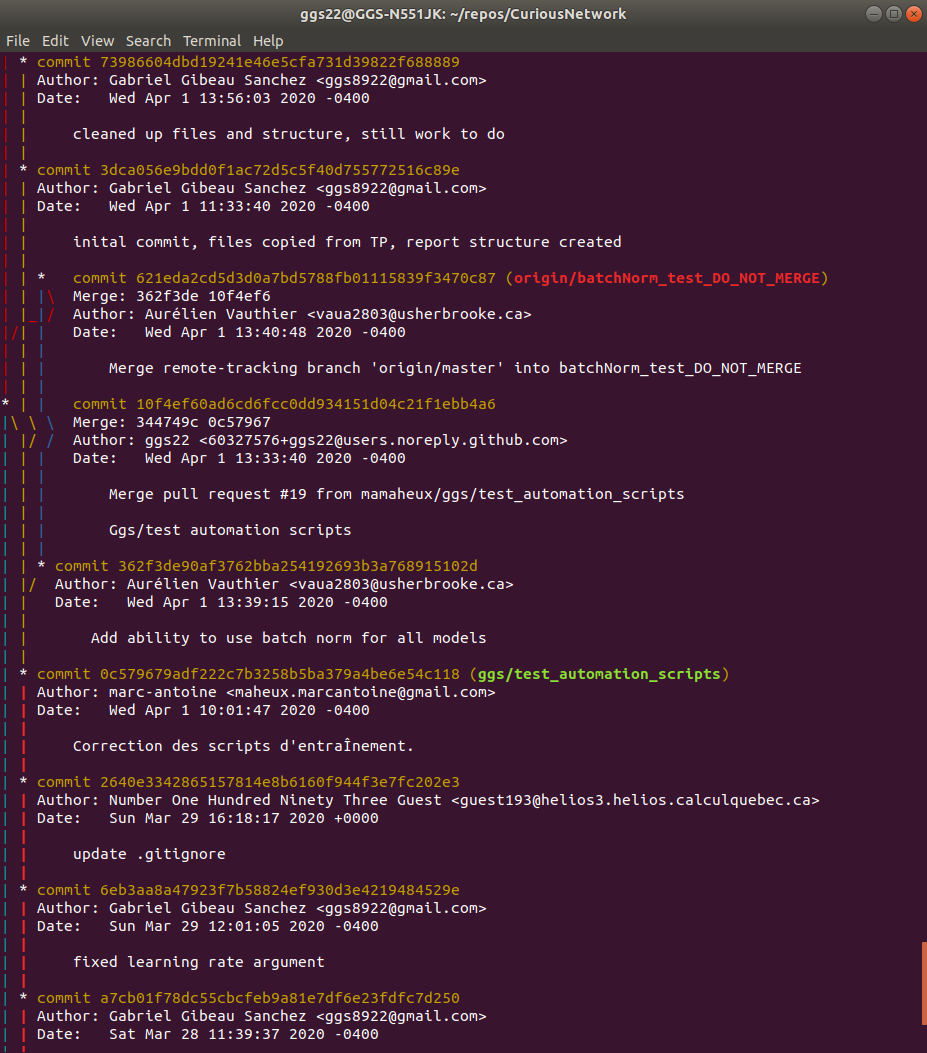
\includegraphics[width=15cm]{images/git_graph.png}
        \caption{Apperçu de l'arborescence du Git}
        \label{fig:git_graph}
    \end{figure}